\documentclass[a4paper, 11pt, normalem]{report}

\usepackage{../../../LaTeX-Templates/Notes}
\usepackage{subfiles}

\title{Statistical Physics \vspace{-20pt}}
\author{Prof Stewart Clark}
\date{\vspace{-15pt}Michaelmas Term 2018}
\rhead{\hyperlink{page.1}{Contents}}
\lhead{M. Rossetter}

\begin{document}

\maketitle
\tableofcontents

\chapter{}
\section{Introduction}
We use probability theory with large numbers to gain insight into real systems.
With N large, we get "information overload" when looking at each particle.
Interference effects from Quantum Mechanics canle out for large N, e.g.
\begin{align}
    |\alpha\psi_1 + \beta\psi_2|^2 &= |\alpha\psi_1|^2 + |\beta\psi_2|^2 + \underbrace{\alpha\psi_1\beta\psi_2 + \beta\psi_2\alpha\psi_1}_{\to 0 \text{ for large N}}
\end{align}

\section{Probability}
A summary:
\begin{itemize}
    \item P(A or B) = P(A) + P(B) for independent events A and B
    \item P(A and B) = P(A)P(B)
    \item Counting events: the number of ways of splitting N objects into 2 piles of size r and (N-r) is
        \begin{equation}
            \begin{pmatrix} N \\ r \end{pmatrix} = \frac{N!}{r!(N-r)!}
        \end{equation}
\end{itemize}

\section{Probability}
Let's have a system containing three objects which can have spin up or down.
Will create a distribution of 1/8, 3/8, 3/8, 1/8, of likelihood of being in a state of All Up, 2 Up One Down, 2 Down One Up, All Down.

\section{Distributions}
\subsection{Discrete}
\begin{itemize}
    \item A variable x can take a number of specific discrete values, $\{x_1, x_2, \dots, x_n\}$, and let the probability of each be $p_i$.
    \item Normalisation gives $\sum_i p_i = 1$.
    \item Mean, $\langle x\rangle = \bar{x} = \sum_i p_ix_i$.
    \item Variance, $\sigma^2 = \bar{x^2} - \bar{x}^2 = \sum_i p_ix_i^2 - \left(\sum_i p_ix_i\right)^2$
    \item Standard deviation, $\sigma$
\end{itemize}

\subsection{Binomial distribution}
This applies when a system has two likely outcomes of probability - p and (1-p).
If we have N trials, then the probability of event p occurring k times ((1-p) occurring (N-k) times) is
\begin{equation}
    P_N(k) = \frac{N!}{k!(N-k)!}p^k(1-p)^{N-k}.
\end{equation}
The normalisation is
\begin{equation}
    \sum_{k=0}^{N} P_N(k) = 1
\end{equation}
and the variance is
\begin{equation}
    \sigma^2 = Np(1-p)
\end{equation}

\subsection{Continuous distribution}
When a variable x takes on any value, $-\infty\leq x <\infty$ (or any range within), then the probability that x equals some value $x_0$ does not make sense.
Instead probability is found in a range, $a\leq x\leq b$, so the continuous distribution is $f(x)$, then,
\begin{equation}
    P(a\leq x\leq b) = \int_{a}^{b} f(x)\,dx
\end{equation}
and the normalisation,
\begin{equation}
    \int_{-\infty}^{\infty} f(x)\,dx = 1.
\end{equation}

A common continuous distribution is the Normal (Gaussian) distribution which is
\begin{equation}
    f(x) = \frac{1}{\sigma\sqrt{2\pi}}e^{-(x-\mu)^2/2\sigma^2}
\end{equation}
\begin{itemize}
    \item $\sigma$ essentially changes the width of the distribution
    \item $\mu$ shifts the centre of the distribution to $x=\mu$
\end{itemize}

\section{Probabilities}
If we perform an experiment N times and event i occurs $n_i$ times, then the frequency of occurrence is $F(n_i, N) = \frac{n_i}{N}$.
Now if we take N copies of the experiment, and perform it once on each experiment, does is yield the same result?
If the experiment is probabilistic, i.e. every experiment, then no.
TO make sense of this, we introduce probability as
\begin{equation}
    P_{n_i} = \lim_{N\to\infty} F(n_i, N)
\end{equation}
When we do this, the above two statements mean the same thing and it is known as the ergodic hypothesis.

\chapter{}
Thermodynamics is very powerful and provides information on bulk systems - it provides minimal information.
Microscopic predictions give information about every particle in the system (subject to level of theory, e.g. classical or qm); this leads to information overload.

\section{Important Definitions}
\begin{itemize}
    \item Macrostate/ensembles: specification of the state of a system based on macroscopic properties, e.g. N - particle number, V - volume, U - energy, T - temperature, p - pressure, M - magnetisation, B - magnetic field, etc.
        \begin{itemize}
            \item Constant particle number, energy, volume (N,U,V ensemble); this is the microcanonical ensemble.
            \item Constant particle number, temperature, volume (N,T,V ensemble); this is the canonical ensemble.
            \item Constant chemical potential, temperature, volume ($\mu$,T,V ensemble); this is the grand canonical ensemble.
        \end{itemize}
    \item Microstate: complete specification of the state of the system, consistent with theory, i.e. what every particle is doing.
\end{itemize}
A macrostate has a very large number of microstates, $\approx N!$.
We must assign likelihoods (probabilities) of any particle being in any state.
In the microcanonical ensemble, we can assign probabilities - as energy is not changing, then the probabilities must be equal.

We need to figure out how to count the microstates - we define distributions.

\begin{example}
Let's take 4 particles, called A,B,C,D.
Now distribute them amongst some energy levels, $\e_n = 0, \e, 2\e, \dots, n\e$.
If we looks at the microcanonical ensemble (N,U,V) $\to (4,4\e,V)$.

Distribution $D_1$: 3 particles in $\e_0$, 1 particle in $\e_4$ - four configurations of this.
\begin{equation}
    \Omega(D_1) = \frac{4!}{3!1!} = 4
\end{equation}
\begin{table}[H]
\centering
\begin{tabular}{|c||c|c|c|c|c||c|}
    \hline
    Distribution, $D_i$ & $n_0$ & $n_1$ & $n_2$ & $n_3$ & $n_4$ & No. of Microstates, $\Omega(D_i)$ \\
    \hline
    $D_1$ & 3 & 0 & 0 & 0 & 1 & $\frac{4!}{3!1!} = 4$ \\
    $D_2$ & 2 & 1 & 0 & 1 & 0 & $\frac{4!}{2!1!1!} = 12$ \\
    $D_3$ & 1 & 2 & 1 & 0 & 0 & $\frac{4!}{1!2!1!} = 12$ \\
    $D_4$ & 2 & 0 & 2 & 0 & 0 & $\frac{4!}{2!2!} = 6$ \\
    $D_5$ & 0 & 4 & 0 & 0 & 0 & $\frac{4!}{4!} = 4$ \\
    \hline
    Average & $\frac{60}{35}$ & $\frac{40}{35}$ & $\frac{24}{35}$ & $\frac{12}{35}$ & $\frac{4}{35}$ & $\Omega_{tot} = 35$ \\
    \hline
    Probability & 0.43 & 0.29 & 0.17 & 0.09 & 0.03 & \\
    \hline
\end{tabular}
\end{table}
\textbf{Image plot in here}

These are classical particles, so how will they distribute amongst energy levels? Boltzmann distribution appears - $\approx \exp{-\frac{\e}{k_BT}}$.
\end{example}

\chapter{}
From the last example, we see that for the macrostate (N,U,V) that some distributions are more likely than others.
From thermodynamics, remember that the most likely state of a system is the one that maximises entropy.
So, is there a connection between microscopic state probabilities and entropy?
Boltzmann concluded that the number of possible microstates, $\Omega$, leads to entropy, i.e.
\begin{equation}
    S = S(\Omega)
\end{equation}
but what is the form of $S(\Omega)$?
We know for independent systems A and B that the probabilities multiply, i.e. $\Omega_{AB} = \Omega_A\Omega_B$.
However for these two systems, we have entropy $S_A$ and $S_B$ and so
\begin{equation}
    S_{AB} = S_A + S_B.
\end{equation}
Boltzmann noted this and proposed that entropy is given by
\begin{equation}
    S = k_B\ln(\Omega).
\end{equation}
This is the link between microscopic and macroscopic quantities.

Consider Stirling's approximation:
\begin{align}
    \ln(N!) &= \sum_{k=1}^N \ln(k) \approx \int_1^N \ln(k)\,dk \\
            &= [k\ln(k) - k]_1^N \\
    \implies \ln(N!) &\approx N\ln(N) - N
\end{align}

\section{Probable Distributions}
A large number of microstates, $\Omega(n_i)$, corresponds to each distribution when N is large, where $\sum_i n_i = N$ and $\Omega = \sum_i \Omega(n_i)$.
The number of microstates in a distribution is similar to the binomial distribution - the most likely massively dominates over the others.
For large N, we have that
\begin{equation}
    \Omega \approx \Omega\{n^{max}\}.
\end{equation}
We need to seek the most probable distribution - this is the distribution that contains the most microstates, and hence maximises entropy.
We need the distribution satisfying the constraints of constant particle number and constant energy, i.e. $\sum_i n_i = N$ and $\sum_i n_i\e_i = U$.
We want to maximise
\begin{align}
    \Omega(\{n_i\}) &= \frac{N!}{\prod_i n_i!} \\
    S(\{n_i\}) &= k_B\ln\left(\frac{N!}{\prod_i n_i!}\right) \\
    \frac{S(\{n_i\})}{k_B} &= \ln(N!) - \ln\left(\prod_i n_i\right) = \ln(N!) - \sum_i \ln(n_i!) \\
                           &= (N\ln(N) - N) - \sum_i (n_i\ln(n_i) - n_i) \\
                           &= N\ln(N) - \sum_i n_i\ln(n_i) \\
                           &= \sum_i n_i\ln(N) - \sum_i n_i\ln(n_i) \\
                           &= -\sum_i n_i\left[\ln(n_i) - \ln(N)\right] \\
                           &= -\sum_i n_i\ln\left(\frac{n_i}{N}\right)
\end{align}
If we define $p_i = \frac{n_i}{N}$ being the probability of finding $n_i$ particles in state i with energy $\e_i$, then we have
\begin{align}
    \frac{S(\{n_i\})}{Nk_B} &= -\sum_i \frac{n_i}{N}\ln\left(\frac{n_i}{N}\right) \\
    \implies S(\{p_i\}) &= -Nk_B\sum_i p_i\ln(p_i).
\end{align}
The statistical entropy by Boltzmann
\begin{equation}
    S = k_B\ln\Omega \geq 0
\end{equation}
and also,
\begin{equation}
    S(\{p_i\}) = -Nk_B\sum_i p_i\ln(p_i).
\end{equation}
This is the link between macroscopic and microscopic entropy.
For probability, this means that the system is in the distribution that maximises entropy, most of the time.

\chapter{}
\section{Method of Lagrange Multipliers}
\begin{align}
    \frac{\p}{\p n_i}&\left[N\ln(N) - \sum_i n_i\ln(n_i) - \alpha\sum_i n_i - \beta\sum_i n_i\e_i\right] = 0 \\
    \implies &0 - \ln(n_i) - 1 - \alpha - \beta\e_i = 0 \\
    \implies & \ln(n_i) = \underbrace{-1 -\alpha}_{A} -\beta\e_i \\
    \implies &n_i = e^Ae^{-\beta\e_i}
\end{align}
These are the $n_is$ that maximise $S(\{n_i\})$.
\begin{align}
    N &= \sum_i n_i = \sum_i e^Ae^{-\beta\e_i} \\
    \implies e^A &= \frac{N}{\sum_i e^{-\beta\e_i}} = \frac{N}{Z} \\
    Z &= \sum_i e^{-\beta\e_i} \\
    \implies n_i &= \frac{N}{Z}e^{-\beta\e_i} \\
    p_i &= \frac{n_i}{N} = \frac{e^{-\beta\e_i}}{Z}
\end{align}
The quantity Z is known as the partition function - coming from the Lagrange multiplier that fixed N.
What about $\beta$?
\begin{equation}
    U = \sum_i n_i\e_i = \frac{N}{Z}\sum_i \e_ie^{-\beta\e_i}
\end{equation}
Now take the derivative with of Z with respect to $-\beta$, giving
\begin{align}
    -\frac{dZ}{d\beta} &= -\frac{d}{d\beta} \sum_i e^{-\beta\e_i} = \sum_i \e_i e^{-\beta\e_i} \\
    U &= -\frac{N}{Z}\frac{dZ}{d\beta} = -N\frac{d}{d\beta}\ln(Z)
\end{align}
If we know U then we get Z or vice versa.
Actually, this expression is valid in other ensembles, e.g. (N,T,V) then if we know Z, we can get U.

Is there a physicaly interpretation of $\beta$?
Let's take the thermodynamic expression $F = U - TS$.
In statistical physics, we've dealt with U and S.
So temperature is
\begin{equation}
    \frac{1}{T} = \frac{\p S}{\p U}\bigg|_V,
\end{equation}
and we already know U and S.

Consider 2 systems, A and B, where we can exhange energy but not particles and are otherwise isolated.
They contain $N^A$ and $N^B$ particles with $N = N^A + N^B$.
The combined system is the microcanonical ensemble (N,U,V) and has energy levels $\e_i^A$ and $\e_i^B$.
The particles have distributions $\{n_i^A\}$ and $\{n_i^B\}$.
Entropy, $S = S^A + S^B$, and so
\begin{align}
    \frac{S^A}{k_B} &= N^A\ln(N^A) - \sum_i n_i^A\ln(n_i^A) \\
    \frac{S^B}{k_B} &= N^B\ln(N^B) - \sum_i n_i^B\ln(n_i^B)
\end{align}
At thermal equilibrium, we are in the distribution that maximises entropy.
With constraints, we have
\begin{multline}
    -\alpha\sum_i n_i^A - \alpha'\sum_i n_i^B - \left[N^A\ln(N^A) + \sum_i n_i^A\ln(n_i^A) + N^B\ln(N^B) + \sum_i n_i^B\ln(n_i^B)\right] \\ -\beta\left[\sum_i n_i^A\e_i^A + \sum_i n_i^B\e_i^B\right]
\end{multline}
We want to maximise this with respect to $n_i^A$ and $n_i^B$.

\chapter{}
From last time:

To maximise, we take the derivatives:
\begin{align}
    \frac{\p}{\p n_i^A} &\to 0 \\
    \frac{\p}{\p n_i^B} &\to 0
\end{align}
The maths is identical to the example of one system.
We get:
\begin{align}
    \frac{n_i^A}{N^A} &= \frac{e^{-\beta\e_i^A}}{Z^A}, Z^A = \sum_i e^{-\beta\e_i^A} \\
    \frac{n_i^B}{N^B} &= \frac{e^{-\beta\e_i^B}}{Z^B}, Z^B = \sum_i e^{-\beta\e_i^B}
\end{align}
Note that both systems have a Boltzmann like probability with the same $\beta$.
In thermodynamics, such a system would have the same T, i.e. $\beta$ and T are related.

Let's let system A contain just one particle, and hence B contains $N-1$ particles.
The system "AB" is in the (N,U,V) macrostate (microcanonical ensemble).

THe probability of any particle being in the state i with energy $\e_i$ is
\begin{equation}
    p_i = \frac{e^{-\beta\e_i}}{Z}.
\end{equation}

The probability of the single particle in A being in state i is
\begin{equation}
    p_i^A = \frac{\Omega(\e_i)}{\sum_i \Omega(\e_i)}
\end{equation}

The energy of system B will be $U - \e_i$ and $\Omega(\e_i) = 1$, and the particles in B will be distributed with energy $U - \e_i$.
\begin{align}
    S^A &= 0 \;\because\; \ln(1) = 0 \\
    S^B &= k_B\ln(\Omega(\{\e_i\}))
\end{align}
But we know
\begin{align}
    \frac{1}{T} = \frac{\p S}{\p U}\bigg|_V &= -k_B\frac{\p}{\p U} (\ln\Omega(\e_i)) \\
                                            &= -k_B\frac{\p}{\p \e_i} \ln\Omega(\e_i)
\end{align}
Let's integrate:
\begin{align}
    \ln\Omega(\e_i) &= -\frac{\e_i}{k_BT} + cst \\
    \implies \Omega(\e_i) &= Ce^{-\e_i/k_BT}
\end{align}
Comparing to previously (Boltzmann expressions), we have
\begin{equation}
    \beta = \frac{1}{k_BT}.
\end{equation}

\section{Free Energy}
We have
\begin{align}
    p_i &= \frac{e^{-\e_i/k_BT}}{Z} \\
    \implies \ln(p_i) &= \frac{-\e_i}{k_BT} - \ln(Z)
\end{align}
For entropy, we know that
\begin{align}
    S &= -Nk_B\sum_i p_i\ln(p_i) \\
      &= Nk_B\sum_ip_i\left(\frac{\e_i}{k_BT} + \ln(Z)\right)
\end{align}
But
\begin{align}
    U &= N\sum_i p_i\e_i \\
    \implies U - TS &= -Nk_BT\ln(Z_{tot})
\end{align}
This is the Helmholtz Free Energy, which is the ability to do work.

The partition function is the free energy - what we can do work with in thermodynamics.

\section{Statistical Physics and Thermodynamics}
We can write
\begin{equation}
    \beta = \frac{1}{k_BT}
\end{equation}
so that it is easier to note how exponentials change.
\begin{align}
    \frac{\p}{\p T} &= \frac{\p}{\p\beta}\frac{\p\beta}{\p T} \\
    \frac{\p\beta}{\p T} &= -\frac{1}{k_BT^2} \\
    \implies \frac{\p}{\p\beta} &= -k_BT^2\frac{\p}{\p T}
\end{align}

\begin{itemize}
    \item Helmholtz Free Energy,
        \begin{equation}
            F = -Nk_BT\ln(Z)
        \end{equation}
    \item Energy,
        \begin{align}
            U &= -N\left[\frac{\p}{\p\beta}\ln(Z)\right]_V \\
              &= Nk_BT^2\left[\frac{\p}{\p T}\ln(Z)\right]_V
        \end{align}
    \item Entropy,
        \begin{equation}
            S = \frac{1}{T}(U-F), S = S(Z)
        \end{equation}
    \item All other thermodynamic properties in terms of Z follow, e.g. heat capacity,
        \begin{equation}
            C_V = \left(\frac{\p U}{\p T}\right)_V
        \end{equation}
\end{itemize}

\chapter{}
A system of one dimensional harmonic oscillators has energy levels:
\begin{equation}
    \e_n = \left(n+\frac{1}{2}\right)\hbar\om.
\end{equation}
Calculate its partition function:
\begin{align}
    Z &= \sum_{n=0}^\infty e^{-\beta\e_n} = \sum_{n=0}^{\infty} e^{-\beta(n+1/2)\hbar\om} \\
      &= e^{-\beta\hbar\om/2}\sum_{n=0}^\infty e^{-\beta n\hbar\om} \\
      &= e^{-\beta\hbar\om/2}\left((e^{-\beta\hbar\om})^0 + (e^{-\beta\hbar\om})^1 + (e^{-\beta\hbar\om})^2 + \dots\right)
\end{align}
THis is just a geometric series in $e^{-\beta\hbar\om}$ so we get
\begin{equation}
    Z = \left[\frac{1}{1 - e^{-\beta\hbar\om}}\right]e^{-\beta\hbar\om/2}
\end{equation}
We now have the partition function of the system in terms of $\beta$ (or T).
The free energy contatins $\ln(Z)$, so
\begin{align}
    \ln(Z) &= \ln\left(\frac{e^{-\beta\hbar\om/2}}{1-e^{-\beta\hbar\om}}\right) \\
           &= -\frac{\beta\hbar\om}{2} - \ln\left(1 - e^{-\beta\hbar\om}\right)
\end{align}
Hence, the Helmholtz energy is
\begin{align}
    F &= -\frac{N\ln(Z)}{\beta} \\
      &= \frac{N\hbar\om}{2} + \frac{N}{\beta}\ln\left(1 - e^{-\beta\hbar\om}\right)
\end{align}

For the internal energy,
\begin{equation}
    U = -N\frac{\p \ln{Z}}{\p \beta},
\end{equation}
we need the $\frac{\p}{\p\beta}$ derivative, i.e.
\begin{align}
    \frac{\p}{\p\beta} &= -\frac{\hbar\om}{2} - \frac{\hbar\om e^{-\beta\hbar\om}}{1 - e^{\beta\hbar\om}} \\
                       &= -\frac{\hbar\om}{2} - \frac{\hbar\om}{e^{\beta\hbar\om} - 1}
\end{align}
Hence, we get
\begin{align}
    U &= \frac{N\hbar\om}{2} + \frac{N\hbar\om}{e^{\beta\hbar\om} - 1} \\
      &= N\hbar\om\left(\frac{1}{2} + \frac{1}{e^{\beta\hbar\om} -1}\right)
\end{align}

For entropy,
\begin{align}
    S &= \frac{U - F}{T} = k_B\beta(U - F) \\
      &= k_B\beta \left[N\hbar\om\left(\frac{1}{2} + \frac{1}{e^{\beta\hbar\om} - 1}\right) - \frac{N\hbar\om}{2} - \frac{N}{\beta}\ln\left(1 - e^{-\beta\hbar\om}\right)\right] \\
      &= Nk_B\left[\frac{\beta\hbar\om}{e^{\beta\hbar\om}} - \ln\left(1 - e^{-\beta\hbar\om}\right)\right]
\end{align}

Now obtain the specific heat of the system at constant volume,
\begin{align}
    C_V &= \frac{\p U}{\p T}\bigg|_V = -k_B\beta^2 \frac{\p U}{\p \beta}\bigg|_V \\
        &= \frac{Nk_B(\beta\hbar\om)^2e^{\beta\hbar\om}}{\left(e^{\beta\hbar\om}-1\right)^2}
\end{align}
Plot the results:
\begin{enumerate}
    \item
        \begin{equation}
            U(T) = \frac{1}{2} + \frac{1}{e^{1/T} - 1}
        \end{equation}
        This starts at $\frac{1}{2}$ and increases non-linearly.
    \item
        \begin{equation}
            S(T) = \frac{1/T}{e^{1/T} - 1} - \ln(1 - e^{-1/T})
        \end{equation}
        Starts at zero and increases non-linearly.
\end{enumerate}

\begin{example}
    Localised $\frac{1}{2}$-spins in a magnetic field.
    If the spins have magnetic moment $\mu$ in a field B, then the energy of spins parallel to B is $-\mu B$ and the energy of the spins anti-parallel to B is $+\mu B$.
    Calculate the partition function of the system.

    We have a two-level system, so introduce notation:
    \begin{align}
        \e_0 &= -\mu B = -\frac{\e}{2} \\
        \e_i &= +\mu B = +\frac{\e}{2}
    \end{align}
    So the partition function is
    \begin{align}
        Z &= \sum_{n=0}^1 e^{-\beta\e_n} = e^{-\beta\e/2} + e^{\beta\e/2}
    \end{align}
\end{example}

\chapter{}
Consider from last time:
\begin{equation}
    Z = e^{-\beta\e/2} + e^{\beta\e/2}
\end{equation}
Probability of finding particle in state $\e_i$ is 
\begin{align}
    p_0 &= \frac{e^{-\beta\e/2}}{e^{\beta\e/2}\left(1 + e^{-\beta\e}\right)} = \frac{e^{-\beta\e}}{1 + e^{-\beta\e}} \\
    p_1 &= \frac{e^{\beta\e/2}}{e^{\beta\e/2}\left(1 + e^{-\beta\e}\right)} = \frac{1}{1 + e^{-\beta\e}}
\end{align}
$p_0$ starts at 0 for low T and approaches $\frac{1}{2}$ as T increases, and opposite for $p_1$.

The magnetisation per particle is the average magnetic moment, i.e.
\begin{equation}
    \frac{M}{N} = p_0(-\mu) + p_1(+\mu) = \mu \frac{1 - e^{-\beta\e}}{1 + e^{-\beta\e}} = \mu\tanh\left(\frac{\beta\e}{2}\right)
\end{equation}
Magnetisation decreases non-linearly with temperature.

For energy, we need $\ln(Z)$, i.e.
\begin{align}
    \ln(Z) &= \ln\left[e^{\beta\e/2}\left(1 + e^{-\beta\e}\right)\right] \\
           &= \frac{\beta\e}{2} + \ln\left(1 + e^{-\beta\e}\right)
\end{align}
We also need
\begin{align}
    \frac{\p}{\p \beta}\ln(Z) &= \frac{\e}{2} - \frac{\e e^{-\beta\e}}{\left(1 + e^{-\beta\e}\right)}
\end{align}
Hence, internal energy,
\begin{align}
    U &= -N\left[\frac{\p \ln(Z)}{\p \beta}\right]_V  \\
      &= -N \left[\frac{\e}{2} - \frac{\e e^{-\beta\e}}{1 + e^{-\beta\e}}\right]
\end{align}
and specific heat, 
\begin{align}
    C_V &= \left[\frac{\p U}{\p T}\right]_V = -k_B\beta^2\left[\frac{\p U}{\p \beta}\right]_V \\
        &= -Nk_B (\beta\e)^2 \frac{e^{-\beta\e}}{\left(1 + e^{-\beta\e}\right)^2}
\end{align}

We also have free energy and entropy:
\begin{align}
    F &= -\frac{N}{\beta}\ln(Z) = -\frac{N\e}{2} - \frac{N}{\beta}\ln\left[1 + e^{-\beta\e}\right] \\
    S &= k_B\beta (U - F) = Nk_B\left[\frac{\beta\e e^{-\beta\e}}{1 + e^{-\beta\e}} - \frac{N}{\beta}\ln\left(1 + e^{-\beta\e}\right)\right]
\end{align}
Plotting entropy vs temperature shows a faster increasing curve for low B than for high B. 
\begin{itemize}
    \item For the same temperature we can move from low B to high B.
        As we increase the B field, then the spins will begin to align, hence entropy decrease.
        The system will change energy, $T\Delta S$.
    \item For the same entropy, can move from high B to low B. 
        We have no change in entropy, $\Delta S = 0$, hence no change in heat, howver the temperature changes, $T_h \to T_l$.
\end{itemize}

We had 
\begin{align}
    S &= Nk_B\left[\frac{\frac{2\mu B}{k_B T}e^{-2\mu B/k_BT}}{1 + e^{-2\mu B/k_BT}} + \ln\left(1 + e^{-2\mu B/k_BT}\right)\right]
\end{align}
In here, $\frac{B}{T}$ appears, therefore is $\Delta S$ is zero, then $\frac{B}{T}$ is constant, i.e.
\begin{align}
    \frac{B_h}{T_h} &= \frac{B_l}{T_l} \\
    \implies T_l &= \frac{B_l}{B_h}T_h
\end{align}
So as we vary B with $\Delta S = 0$, we vary T.
This is called adiabatic demagnetisation.

\chapter{}
In statistical physics, we need the energies of the states and their degeneracies.
In discrete systems, this is obvious.
However in systems where energies come in a continuum, we need the density of states. 
We seek the density $g(\e)$ of states in the range $\e \to \e+d\e$. 
Also, we often have relationships between energy and momentum, e.g. in 1D ISW, $E = \frac{\hbar^2k^2}{2m}$ (momentum is $\hbar k$), so we sometimes seek $g(k)$ instead.

Let $n(k)$ be the number of independent solutions with $k \in 0 \to k_0$ and similar for $n(k+\delta k)$.
Therefore, 
\begin{align}
    g(k)\;\delta k &= n(k+\delta k) - n(k) \\
                   &= \frac{n(k+\delta k) - n(k)}{\delta k}\delta k \\
                   &= \frac{dn}{dk}\delta k
\end{align}

\begin{example}
    In the 3D ISW, we had solutions, 
    \begin{align}
        \Psi(x,y,z) &= \sin(k_xx)\sin(k_yy)\sin(k_zz)
    \end{align}
    with 
    \begin{align}
        k_x &= \frac{\pi}{a}n & k_y &= \frac{\pi}{a}m & k_z &= \frac{\pi}{a}l & n,m,l &\in \N
    \end{align}
    Let's count states.
    If $n(k)$ is the number of independent states, we have
    \begin{align}
        n(k) &= \frac{\text{Volume in 3D k-space (in all positive octant)}}{\left(\frac{\pi}{a}\right)^3} \\
             &= \frac{1}{8}\times \frac{4}{3}\pi k^3 \left(\frac{a}{\pi}\right)^3
    \end{align}
    Hence, 
    \begin{align}
        g(k)\;\delta k &= \frac{dn(k)}{dk} = \frac{a^3}{(2\pi)^3}4\pi k^2
    \end{align}
    Other notes: 
    \begin{itemize}
        \item If we include spin, then multiply $n(k)$ by 2.
    \end{itemize}
    For energy, we have 
    \begin{align}
        E &= \frac{\hbar^2 k^2}{2m} \\
        k &= \left(\frac{2mE}{\hbar^2}\right)^{1/2} \\
        \frac{dk}{dE} &= \frac{1}{2} \left(\frac{2mE}{\hbar^2}\right)^{-1/2} \left(\frac{2m}{\hbar^2}\right) \\
                               &= \frac{1}{2}\frac{1}{k}\frac{2m}{\hbar^2} \\
        dk &= \frac{m}{\hbar^2 k}dE \\
        g(E)\,dE &= a^3 \frac{2\pi}{\hbar^3} (2m)^{3/2} E^{1/2}\;dE \\
        g(E) &\approx E^{1/2}
    \end{align}
    This is the energy density of states.
\end{example}

\section{More distributions}
For N particles, a large number of microstates, $\Omega$, correspond to each distribution $\{n_1,n_2,n_3,\dots\}$ and we seek the one that is largest.
The most probable distribution is the one which contains the most microstates. 
So we find the particular $\{n_1,n_2,n_3,\dots\}$ with constraints $\sum_j n_j = N$ (constant particle number) and $\sum_j n_j\e_j = U$ (constant energy), for which
\begin{equation}
    \Omega(\{n_j\}) = \frac{N!}{\prod_j n_j!}
\end{equation}
is maximum.

What changes if for state 1, we allow $g_1$ particles in it, i.e. $g_1$ degeneracy?
There are more microstates - what was previously $n_1$ can now be $g_1$-fold degenerate, i.e.
\begin{equation}
    \Omega(\{n_j\}) = \frac{N!}{\prod_j n_j!}\times g_1^{n_1}.
\end{equation}
Let's now let state 2 be $g_2$-fold degenerate, giving
\begin{equation}
    \Omega(\{n_j\}) = \frac{N!}{\prod_j n_j!}\times g_1^{n_1} \times g_2^{n_2}.
\end{equation}
It is now straightforward to generalise such that state j is $g_j$-fold degenerate. 
\begin{equation}
    \Omega(\{n_j\}) = N! \prod_j \frac{g_j^{n_j}}{n_j!},
\end{equation}
where $n_j$ is the number of distinguishable particles in the state with energy $\e_j$ which is $g_j$-fold degenerate.
We now want to maximise this with respect to the $n_j$s.
So we want to maximise entropy under the constraints given above: 
\begin{align}
    \frac{S}{k_B} &= \ln\left[N!\prod_j \frac{g_j^{n_j}}{n_j!}\right] \\
                  &= \sum_j \left[n_j\ln(g_j) - \ln(n_j!)\right] + \ln(N!) \\
                  &\approx \sum_j \left[n_j\ln(g_j) - n_j\ln(n_j) + n_j\right] + \ln(N!)
\end{align}
Now maximise with respect to the $n_j$, i.e. do $\frac{\p}{\p n_j}$ on above with Lagrange multipliers and set to zero:
\begin{align}
    \frac{\p}{\p n_j} \left[\sum_j \left(n_j\ln(g_j) - n_j\ln(n_j) + n_j - \alpha n_j - \beta n_j\e_j\right)\right] &= 0 \\
    \ln(g_j) - \ln(n_j) - 1 + 1 - \alpha - \beta\e_j &= 0 \\
    \ln\left(\frac{g_j}{n_j}\right) &= \alpha + \beta\e_j \\
    \frac{n_j}{g_j} &= e^{-\alpha}e^{-\beta\e_j}
\end{align}

\chapter{}
We have classical, distinguishable particles
\begin{align}
    \Omega(\{n_i\}) &= N!\prod_i \frac{g_i^{n_i}}{n_i!} \\
    \frac{n_i}{g_i} &= e^{-\alpha}e^{-\beta \e_k}
\end{align}
Leads to Maxwell-Boltzmann distribution
\begin{equation}
    f_{MB}(\e_j) = e^{-\alpha}e^{\beta \e_j}
\end{equation}
As previously noted, $\alpha$ is determined from fixed N ($\int f_{MB}(\e)\;d\e = N$), and $\beta = \frac{1}{k_BT}$.

This is the distribution of particles which are "classical" (distinguishable) at temperature, T. 

What about indistinguishable particles?
Recall
\begin{align}
    \hat{S}\Psi(r_1,r_2) &= \Psi(r_2,r_1) 
\end{align}

So we have two sets of particles:
\begin{itemize}
    \item Fermions
        \begin{equation}
            \Psi(r_1,r_2) = -\Psi(r_2,r_1)
        \end{equation}
    \item Bosons
        \begin{equation}
            \Psi(r_1,r_2) = \Psi(r_2,r_1)
        \end{equation}
\end{itemize}
For fermions, $\Psi(r,r) = 0$ $\implies$ \emph{Pauli Exclusion Principle.}

\section{Fermion Statistics}
Each single particle state will either be occupied or unoccupied. 
So with degeneracy, $g_j$, for a state with energy, $\e_j$, we want the number of ways the $g_j$ states can be put into two piles (occupied and unoccupied).

\begin{itemize}
    \item If there are $n_j$ particles in states, then there are $g_j - n_j$ unoccupied states.
    \item For a state with energy, $\e_j$, we get
        \begin{equation}
            \Omega(\e_j) = \frac{g_j!}{n_j!(g_j-n_j)!}
        \end{equation}
        This is the jth state, hence for all states we get
        \begin{equation}
            \Omega_{FD} = \prod_j \frac{g_j!}{n_j(g_j-n_j)!}
        \end{equation}
\end{itemize} 
Maximising the entropy under the constraints of fixed particle number fixed energy:
\begin{align}
    \frac{S}{k_B} = \ln(\Omega) &= \ln\left(\prod_j \frac{g_j!}{n_j!(g_j-n_j)!}\right) \\
                                &= \sum_j\left[\ln(g_j!) - \ln(n_j!) - \ln((g_j-n_j)!)\right] \\
                                &= \sum_j\left[g_j\ln(g_j) - g_j - (n_j\ln(n_j) - n_j) - ((g_j-n_j)\ln(g_j-n_j) - (g_j-n_j))\right] \\
                                &= \sum_j\left[g_j\ln(g_j) - n_j\ln(n_j) - (g_j-n_j)\ln(g_j-n_j)\right]
\end{align}
Introducing the usual Lagrange multipliers and maximising with respect to particle number - this is a binomial distribution so we don't need to do a mathematical check as to whether it's a maximum or a minimum.
\begin{gather}
    \frac{\p}{\p n_j}\left[\sum_j\left(g_j\ln(g_j) - n_j\ln(n_j) - (g_j-n_j)\ln(g_j-n_j)\right) - \alpha\sum_jn_j - \beta\sum_jn_j\e_j\right] = 0 \\
        \frac{\p}{\p n_j}[\cdots] = -\ln(n_j) -1 + \ln(g_j-n_j)+1-\alpha-\beta\e_j = 0 \\
        \ln\left(\frac{g_j}{n_j} - 1\right) = \alpha + \beta\e_j \\
        \frac{n_j}{g_j} = \frac{1}{e^{\alpha}e^{\beta\e_j}+1}
\end{gather}
This is the Fermi-Dirac distribution function:
\begin{equation}
    f_{FD} = \frac{1}{e^{\alpha}e^{\beta\e_j}+1}
\end{equation}

\section{Bosons}
How to count microstates? Here there is no restriction on state occupancy within the $g_j$ degenerate state with energy $\e_j$.
It can accomodate any number of particles $n_j$.

Rather than putting the particles in boxes, let's imagine we have all the particles lined up and we arrange the "partitions" between groups of particles. 
So we have objects $n_j+(g_j-1)$ and we split them into groups of $n_j$ and $(g_j-1)$, giving for energy state $\e_j$,
\begin{align}
    \Omega(\e_j) &= \frac{(n_j+g_j-1)!}{n_j!(g_j-1)!} \\ 
                 &\approx \frac{(n_j+g_j)!}{n_j!g_j!} \\
\end{align}
Therefore for all states, we get the total number of microstates as
\begin{equation}
    \Omega_{BE} = \prod_j \frac{(n_j+g_j)!}{n_j!g_j!}
\end{equation}


\chapter{}
\section{Boson Statistics}
\begin{align}
    \Omega_{BE} &= \prod_j \frac{(n_j + g_j)!}{n_j!g_j!} \\
    \frac{S}{k_B} &= \ln\left[\prod_j \frac{(n_j+g_j)!}{n_j!g_j!}\right] = \sum_j \left[\ln(n_j + g_j)! - \ln(n_j!) - \ln(g_j!)\right] \\
                  &= \sum_j \left[(n_j+g_j)\ln(n_j+g_j) - (n_j+g_j) - (n_j\ln(n_j) - n_j) - (g_j\ln(g_j) - g_j)\right] \\
                  &= \sum_j \left[(n_j+g_j)\ln(n_j+g_j) - n_j\ln(n_j) - g_j\ln(g_j)\right]
\end{align}
So maximise this with constraints on particle nunber and energy (as usual). 
With Lagrange multipliers, we have
\begin{gather}
    \frac{\p}{\p n_j}\left[\sum_j\left[(n_j+g_j)\ln(n_j+g_j) - n_j\ln(n_j) - g_j\ln(g_j) - \alpha n_j - \beta n_j\e_j\right]\right] = 0 \\
    \ln(n_j+g_j) + 1 - \ln(n_j) - 1 - \alpha - \beta\e_j = 0 \\
    \ln(\frac{g_j}{n_j} + 1) = \alpha + \beta\e_j \\
    \frac{n_j}{g_j} = \frac{1}{e^{\alpha}e^{\beta\e_j}-1}
\end{gather}
This is the Bose-Einstein distribution function, i.e.
\begin{align}
    f_{BE}(\e) &= \frac{1}{e^{\alpha}e^{\beta\e}-1}
\end{align}

So, after all this work, we finally have the distribution functions for classical particles, fermions, and bosons.
They are:
\begin{align}
    f(\e) &= \frac{1}{e^{\alpha}e^{\beta/k_BT}\begin{cases} +1 & \text{Fermions, Fermi-Dirac} \\ 0 & \text{Classical, Maxwell-Boltzmann} \\ -1 & \text{Bosons, Bose-Einstein} \end{cases}}
\end{align}

\begin{example}
    In the non-quantum limit (this means $n_j \ll g_j$ - sometimes called the dilute limit), do the three sets of statistics become the same?
    \begin{itemize}
        \item Fermions:
            \begin{align}
                \Omega(\e_j) &= \frac{g_j!}{n_j!(g_j-n_j)!} \\
                             &= \frac{\overbrace{1\times2\times3\times\cdots\times(g_j-n_j)}^{(g_j-n_j)!}(g_j-n_j+1)\times\cdots\times g_j}{n_j!(g_j-n_j)!} \approx \frac{g_j^{n_j}}{n_j!}
            \end{align}
        \item Bosons:
            \begin{align}
                \Omega_{BE}(\e_j) &= \frac{(n_j+g_j)!}{n_j!g_j!} \\
                            &= \frac{\overbrace{1\times2\times\cdots\times g_j}^{g_j!}(g_j+1)\times\cdots\times(n_j+g_j)}{n_j!g_j!} \approx \frac{g_j^{n_j}}{n_j!}
            \end{align}
        \item Classical:
            \begin{align}
                \Omega_{MB}(\e_j) &= \frac{g_j^{n_j}}{n_j!}
            \end{align}
    \end{itemize}
    Now we take the product over all states, $\prod_j$ to get the same result. 
    However, if you look back to the classical result, which is for distinguishable particles, we had an extra factor of $N!$.

    So are dilute limit FD or BE equal to MB? \unl{This is called the Gibbs paradox.} (More on this later.)
\end{example}

\section{Thermal Averages}
Let Q be some thermal property. 
When a particle is in a state with energy $\e_j$, that particle has microscopic property $Q_j$.
THe system can best be described by combining all of those microscopic properties, with a weighted average using the distribution function, i.e. the average is
\begin{align}
    \langle Q\rangle &= \frac{1}{N}\sum_j n_jQ_j
\end{align}
We usually don't have $n_j$, but we have the distribution functions. 
We have 
\begin{align}
    n_j &= g_jf_j \\
    f_j &= \frac{N}{Z}e^{-\beta\e_j} \\
    \langle Q\rangle &= \frac{\sum_j g_j e^{-\beta\e_j}Q_j}{\sum_j g_je^{-\beta\e_j}}
\end{align}
In bulk systems, the states become continuous, so sums are written as integrals and we get
\begin{align}
    \langle Q\rangle &= \frac{\ofnt g(\e)e^{-\beta\e}Q(\e)\,d\e}{\ofnt g(\e)e^{-\beta\e}d\e}
\end{align}
Or, in k-space, we have
\begin{align}
    \langle Q\rangle &= \frac{\ofnt g(k)e^{-\beta\e(k)}Q(k)\;dk}{\ofnt g(k)e^{-\beta\e(k)}dk}
\end{align}

\chapter{}
In bulk systems, the states become continuous, so sums are written as integrals and we get
\begin{align}
    \langle Q\rangle &= \frac{\ofnt g(\e)e^{-\beta\e}Q(\e)\,d\e}{\ofnt g(\e)e^{-\beta\e}d\e}
\end{align}
Or, in k-space, we have
\begin{align}
    \langle Q\rangle &= \frac{\ofnt g(k)e^{-\beta\e(k)}Q(k)\;dk}{\ofnt g(k)e^{-\beta\e(k)}dk}
\end{align}
For density of states, we had for a 3D gas, $g(k) \propto k^2$ and $g(\e) \propto \e^{1/2}$.
We also have the partition function, 
\begin{align}
    Z &= \sum_{i\text{ states}} e^{-\beta\e_i} = \sum_{j\text{ energies}} g_je^{-\beta\e_j} \\
      &= \ofnt g(k)e^{-\beta \e(k)}dk = \ofnt g(\e)e^{-\beta\e}d\e
\end{align}


\begin{example}
    The density of states for the 3D dilute gas was
    \begin{align}
        g(k)\;\delta k &= \frac{V}{(2\pi)^2}4\pi k^2\;\delta k \\
        \implies Z &= \frac{V}{(2\pi)^2}4\pi \ofnt k^2e^{-\beta\hbar^2k^2/2m}\,dk \\
        \ofnt x^2e^{-\lambda x^2}\,dx &= \frac{1}{4}\sqrt{\frac{\pi}{\lambda^3}} \\
        \implies Z &= V\left(\frac{2\pi M}{\beta h^2}\right)^{3/2} = \frac{V}{\lambda_D^3} \\
        \lambda_D &= h\sqrt{\frac{\beta}{2\pi M}} = \frac{h}{\sqrt{2\pi Mk_BT}}
    \end{align}
\end{example}
$\lambda_D$ is known as the deBroglie thermal wavelength. 
This is a measure of how "classical" or "quantum" the system is, i.e. how dilute or how dense the system is. 
If $\lambda_D$ is much smaller than interparticle distance, then we are in the dilute (non-quantum) limit.

If we have the density of states as $g(k)$, then we know that $\hbar k = mv$ and $\frac{\hbar^2k^2}{2m} = \frac{1}{2}mv^2$ so we can also obtain $g(v)$.
It gives the number of particles lying between $v$ and $v+\delta v$, so
\begin{align}
    n(v)\;\delta v &= g(v)\;\delta v ~e^{-\alpha}e^{-\beta\e(v)} = Cv^2e^{-\beta mv^2/2}
\end{align}
We can calculate $C$ by noting that 
\begin{align}
    N &= \ofnt n(v)\;dv
\end{align}
Integrating this gives (using earlier integral)
\begin{equation}
    C = 4\pi N\left(\frac{\beta M}{2\pi}\right)^{3/2}.
\end{equation}
We are in the classical limit and note that $h$ has gone. 

\begin{example}[What is the most probable speed of a particle in the 3D box?]
    We maximise $n(v)$ to get the most probable.
    As we increase temperature, the $n(v)$ is more spread out, with a lower peak shifted to the right.
    \begin{align}
        \frac{dn(v)}{dv} &= C\,2ve^{-\beta mv^2/2}\left(1 - \beta \frac{mv^2}{2}\right) = 0 \\
        \implies v_{max} &= \sqrt{\frac{2}{\beta m}}
    \end{align}
    Now consider the mean speed. 
    Using the thermal averages above, we get:
    \begin{align}
        \bar{v} &= \frac{\ofnt v^2e^{-\beta mv^2/2}v\;dv}{\ofnt v^2e^{-\beta mv^2/2}\;dv} \\
                &= \sqrt{\frac{8}{\pi\beta m}}
    \end{align}
    How about RMS speed?
    \begin{align}
        v^2_{RMS} &= \frac{\ofnt v^2e^{-\beta mv^2/2}v^2\;dv}{\ofnt v^2e^{-\beta mv^2/2}\;dv} \\
                  &= \frac{3}{\beta m} \\
        v_{RMS} &= \sqrt{\frac{3}{\beta m}}
    \end{align}
    Note that:
    \begin{itemize}
        \item 
            \begin{align}
                \ofnt x^3e^{-x^2}\,dx &= \frac{1}{2} \\
                \ofnt x^4e^{-x^2}\,dx &= \frac{3}{8}\sqrt{\pi}
            \end{align}
        \item 
            \begin{align}
                \langle E\rangle &= \frac{1}{2}mv^2_{RMS} = \frac{1}{2}m\frac{3}{\beta m} \\
                                 &= \frac{3}{2}k_BT
            \end{align}
            This is \unl{Equipartition} - we get $\frac{1}{2}k_BT$ of energy per degree of freedom.
    \end{itemize}
    What is this system's partition function?
    \begin{align}
        Z &= V\left(\frac{2\pi m}{\beta h^2}\right)^{3/2} = \frac{V}{\lambda_D^3}
    \end{align}
    Hence let's calculate some thermodynamic properties:
    \begin{align}
        U &= -N\frac{\p\ln(Z)}{\p\beta} = \cdots = \frac{3Nk_BT}{2} \\
        F &= -Nk_BT \ln(Z) = \cdots = -Nk_BT(\ln(V) - 3\ln(\lambda_D))
    \end{align}
\end{example}

\chapter{}
For the Maxwell-Boltzmann distribution of a dilute monatomic gas, we had:
\begin{equation}
    Z_1 = V\left(\frac{2\pi m}{\beta h^2}\right)^{3/2}  = \frac{V}{\lambda_D^3},~ \lambda_D = \sqrt{\frac{\beta h^2}{2\pi m}}
\end{equation}
The partition function for N particles appears to be $Z_1^N$.
When using this, we end up with properties such as entropy that are not extensive. 
Instead if we use $\frac{Z_1^N}{N!}$, then we get
\begin{align}
    \ln\left(\frac{Z_1^N}{N!}\right) &= N\ln(Z_1) - \ln(N!) \\
                                     &= N\ln(Z_1) - N\ln(N) + N \\
                                     &= N\left(\ln\left(\frac{Z_1}{N}\right) + 1\right) \\
                                     &= N\left(\ln\left(\frac{V}{N}\right) - 3\ln(\lambda_D) + 1\right)
\end{align}
So for Free Energy and Internal Energy, we have
\begin{align}
    F &= k_BT\ln(Z_N) = -Nk_BT\left[\ln\left(\frac{V}{N}\right) - 3\ln(\lambda_D) + 1\right] \\
    U &= -\frac{\p}{\p\beta}\ln(Z_N) = \frac{3N}{\beta} = \frac{3}{2}Nk_BT
\end{align}
If we had not included the $N!$ term in the partition function, we would have obtained
\begin{align}
    F &= -Nk_BT\left[\ln(V) - 3\ln(\lambda_D)\right]
\end{align}
This is problematic - if we double $N$ and $V$, wouldn't double $F$. 
However, when including $N!$, we see that $N$ and $V$ appear together as $\frac{V}{N}$ and so the "2" in doubling cancels. 
We are being forced to include the $N!$ in counting the "classical" arrangements (microstates).

\begin{example}
    A box containing a partition and $N = N_1 + N_2$ particles in volume $V = V_1 + V_2$. 
    Let the temperature be $T$. 
    The particles in each side are the same (not \emph{identical}), and let $V_1 = V_2 = \frac{V}{2}$ and $N_1 = N_2 = \frac{N}{2}$ (divided in half).
    \begin{align}
        S^1_{classic}\left(\frac{N}{2},\frac{V}{2}\right) + S^2_{classic}\left(\frac{N}{2},\frac{V}{2}\right) &= \frac{3}{2}k_B\frac{N}{2} + \frac{3}{2}k_B\frac{N}{2} + \frac{N}{2}k_B\left[\ln\left(\frac{V}{2}\right) - 3\ln(\lambda_D)\right] + \frac{N}{2}k_B\left[\ln\left(\frac{V}{2}\right) - 3\ln(\lambda_D)\right] \\
                                                                                                              &= \frac{3}{2}k_BN + Nk_B\left[\ln\left(\frac{V}{2}\right) - 3\ln(\lambda_D)\right]
    \end{align}
    We can write similarly for the whole box and see the difference:
    \begin{align}
        S_{classic}(N,V) - S_{classic}\left(\frac{N}{2},\frac{V}{2}\right) &= Nk_B\ln(2)
    \end{align}
    So if we let the gas mix, we get an increase in entropy of $Nk_B\ln(2) > 0$.
    If we put the partition back in, don't we still have the same system?
    But there is an apparent entropy increase.
    The entropy should \unl{not} increase - there is no effective difference between "before" and "after", hence even classically, we need the concept of distinguishable and indistinguishable particles.
\end{example}

\begin{example}[The Diatomic Molecule]
    Describe the Degrees of Freedom:
    \begin{itemize}
        \item Translational (rigid)
        \item Rotational (rigid)
        \item Vibrational
        \item Electronic excitations
    \end{itemize}
    So the partition function from these is
    \begin{align}
        Z &= \sum_{\text{all states}} e^{-\beta\left(E_{elec}+E_{tran}+E_{vib}+E_{rot}\right)} \\
          &= Z_{elec}\frac{Z_{tran}}{N!}Z_{vib}Z_{rot}
    \end{align}
    Note: the $N!$ comes from counting the translational DoFs classically. 
    
    So Free Energy is
    \begin{align}
        F &= -Nk_BT\ln(Z_{elec} - Nk_BT\left[\ln\left(\frac{Z_{tran}}{N!}+1\right)\right] - Nk_BT\ln(Z_{vib}) - Nk_BT\ln(Z_{rot}) \\
        Z_{tran} = \frac{V}{\lambda_D^3} &\implies U_{trans} = \frac{3}{2}Nk_BT \\
                                         &\implies C_V = \frac{3}{2}Nk_B
    \end{align}
    \begin{itemize}
        \item Electronic term:
            \begin{align} 
                Z_{elec} &= e^{-\beta E_0} + e^{-\beta E_1} + e^{-\beta E_2} + \cdots \\
                         &= e^{-\beta E_0}\left[1 = e^{-\beta(E_1-E_0)} + \cdots\right] 
            \end{align}
            For molecules, $E_1-E_0 \approx 10\text{eV}$.
            For scale, $k_BT \approx E_1-E_0 \implies T \approx 10^5\;K$.
            Hence, 
            \begin{align}
                Z_{elec} &\approx e^{-\beta E_0} \\
                \ln(Z_{elec}) &= -\beta E_0
            \end{align}
            So the electronic contribution to the internal energy is
            \begin{align}
                \frac{U}{N} &= -\frac{\p}{\p\beta}\ln(Z) = E_0 \text{ (a constant)}
                \implies C_V^{elec} &= \frac{\p U}{\p T}\bigg| = \frac{\p}{\pi T} E_0 = 0
            \end{align}
        \item Vibrations \\
            We know for a diatomic that $\e_n = \left(n+\frac{1}{2}\right)\hbar\om$ and we know the partition function of this:
            \begin{align}
                Z_{vib} &= \frac{e^{-\beta\hbar\om/2}}{1 - e^{-\beta\hbar\om}}
            \end{align}
    \end{itemize}
\end{example}

\chapter{}

\begin{example}[Ctd]
    \begin{itemize}
        \item Vibrations \\
            We know for a diatomic that $\e_n = \left(n+\frac{1}{2}\right)\hbar\om$ and we know the partition function of this:
            \begin{align}
                Z_{vib} &= \frac{e^{-\beta\hbar\om/2}}{1 - e^{-\beta\hbar\om}} \\
                U_{vib} &= -N\frac{\p\ln(Z_{vib})}{\p\beta} = \frac{N\hbar\om}{2} + \frac{N\hbar\om}{e^{\beta\hbar\om} - 1} \\
                C_V^{vib} &= \frac{\p U}{\p T} = \frac{Nk_B(\hbar\om\beta)^2e^{\beta\hbar\om}}{(e^{\beta\hbar\om} - 1)^2}
            \end{align}
            The $O_2$ molecule vibrates at $62\,$THz - frequency to temperature conversion gives this at around $5000$K. \\
            Now examine the high temperature limit - this means for large n. 
            Evaluate high T partition function:
            \begin{align}
                Z^{high}_{vib} &= e^{-\beta\hbar\om/2}\sum_{n=0}^\infty e^{-\beta\hbar\om n} \approx e^{-\beta\hbar\om/2} \ofnt e^{-\beta\hbar\om n}dn \\ 
                        &= \frac{e^{-\beta\hbar\om/2}}{\beta\hbar\om}
            \end{align}
            \begin{itemize}
                \item \textbf{Note: can convert this sum to integral as the "step size" of 1 in the sum becomes insignificant at higher values - where we are interested for high T.} 
            \end{itemize} 
            \vspace{10pt}
            Hence high T limit of internal energy is 
            \begin{align}
                U^{high}_{vib} &= -N\frac{\p\ln(Z^{high}_{vib})}{\p\beta} = \frac{N\hbar\om}{2} + Nk_BT \\
                C^{high}_{vib} &= \frac{\p U_{vib}^{high}}{\p T} = Nk_B
            \end{align}
        \item Rotations \\
            These are quantised as well, with
            \begin{align}
                L_z &= m\hbar,~ -l \leq m \leq l \\
                L^2 &= l(l+1)\hbar^2, l \in \N
            \end{align}
            If the moment of inertia of the molecule is $I$, then the energy of rotation is 
            \begin{align}
                E &= \frac{L^2}{2I} \\
                Z_{rot} &= \sum_l g_l e^{-\beta\e_l} = \sum_{l=0}^\infty (2l+1) e^{-\beta\hbar^2l(l+1)/"I} = ~? \\
                Z_{rot}^{high} &\approx \ofnt (2l+1)e^{-\beta\hbar^2l(l+1)/2I},~ x = \beta\hbar^2l(l+1)/2I \\
                               &= \frac{2I}{\hbar^2\beta} \\
                \ln(Z_{rot}^{high}) &= \ln(2I) - \ln(\beta\hbar^2) \\
                U_{rot}^{high} &= -N\frac{\p\ln(Z_{rot}^{high})}{\p\beta} = Nk_BT \\
                C_{V,rot}^{high} &= Nk_B,~ T >> T_{rot}
            \end{align}
            Where $T_{rot}$ is a few Kelvin. \\
            In the low temperature limit, we do this by taking the first couple of terms in Z. 
            If $T << T_{rot}$, we have 
            \begin{align}
                Z_{rot}^{low} &= \sum_{l=0}^1 (2l+1)e^{-\beta\hbar^2l(l+1)/2I} \\
                U_{rot}^{low} &= \frac{3N\hbar^2}{I}e^{-\beta\hbar^2/I} \\
                C_{V,rot}^{low} &= 3Nk_B\left(\frac{\beta\hbar^2}{I}\right)^2e^{-\beta\hbar^2/I}
            \end{align}
    \end{itemize}
    So to summarize, the heat capacity of diatomic molecules changes with temperature as first rotational, then vibrational, then electronic degrees of freedom are unlocked.
    \begin{center}
        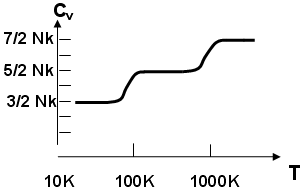
\includegraphics[scale=0.8]{cv.png}
    \end{center}
\end{example}

\section{Fermi-Dirac Systems}
These are systems with half-integer spin, which obey Pauli exclusion. 
The systems can be fundamental (e.g. electrons) or competitive (e.g. atoms) - conduction electrons, liquid $^3$He ($^4$He is a boson), white dwarf starts, protons.

We need to use Fermi-Dirac statistics, i.e.
\begin{align}
    f_{FD}(\e) &= \frac{1}{e^{\alpha}e^{\beta\e} + 1} = \frac{1}{e^{\beta(\e-\mu)}+1},~ e^{\alpha} = e^{-\mu\beta}
\end{align}
Our particle number constraint is equivalent to an energy - adding or removing particles changes the value of $\mu$.
$\mu$ is called the chemical potential, or the Fermi level ($\e_F$).
The distribution $f_FD(\e)$ is the average occupation at energy $\e \to \e+d\e$ and for single particle states, we have
\begin{align}
    f_{FD}(\e_i) &= \frac{n_i}{g_i} \implies 0 \leq f_{FD} \leq 1 
\end{align}
We can calculate the Fermi level (or chemical potential) by:
\begin{align}
    N &= \int_0^{\e_F} g(\e)f_{FD}(\e)\;d\e
\end{align}
This is in the ground state at $T$.

\chapter{}
\section{Fermi-Dirac Systems Ctd}
\begin{wrapfigure}{r}{0.4\textwidth}
    \centering
    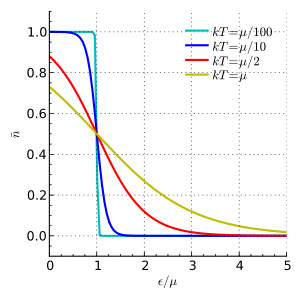
\includegraphics[scale=0.6]{fd.png}
\end{wrapfigure}
For plotting $f_{FD}(\e)$, we get
\begin{align}
    f_{FD}(\e) &= \frac{1}{e^{\beta(\e-\mu)}+1} \\
    f_{FD}(\mu) &= \frac{1}{2} \forall T \\
    \lim_{T\to 0} f_{FD}(\e < \mu) &= 1 \\
    \lim_{T\to 0} f_{FD}(\e > \mu) &= 0 
\end{align}

\begin{example}[At $T=0$, calculate the Fermi level for Fermions in a box of volume, $V$.]
"In a box" means:
\begin{align}
    g(\e)\;d\e &= 2\cdot\frac{2\pi V}{h^3}(2M)^{3/2} \e^{1/2}\,d\e \\
    N &= \ofnt g(\e)\;d\e
\end{align}
But at $T=0$, $f_{FD}(\e)$ is just a step function where the step is at the Fermi level.
Hence, 
\begin{align}
    N &= \int_0^{\e_F} \left(\frac{4\pi V}{h^3}\right)(2M)^{3/2}\e^{1/2}\cdot1\cdot d\e \\
    \implies \e_F &= \frac{h^2}{2M}\left(\frac{3N}{8\pi V}\right)^{2/3}
\end{align}
\end{example}

\subsection{Mathematical Aside}
We will often find integrals of the form
\begin{align}
    \ofnt \frac{\e^{1/2}}{e^{-\beta\e} + 1}\,d\e
\end{align}
Recall that for a $\delta$-function
\begin{align}
    \ifnt \delta(\e-\mu)F(\e)\,d\e &= F(\mu)
\end{align}
But if we had a highly peaked function, $\delta_\sigma$, we have
\begin{align}
    \ifnt \delta_\sigma(\e-\mu)(\e-\mu)^2\,d\e &= \sigma^2 << 1
\end{align}
If we expand $F(\e)$ around $\mu$, then 
\begin{align}
    F(\e) &= F(\mu) + (\e-\mu)F'(\mu) + \frac{1}{2}(\e-\mu)^2F''(\mu) + \cdots 
\end{align}
So we have
\begin{align}
    \begin{split}
        \ifnt \delta_\sigma(\e-\mu)F(\e)\,d\e = F(\mu)\underbrace{\ofnt \delta_\sigma(\e-\mu)\,d\e}_{1} &+ F'(\mu)\underbrace{\ifnt \delta_\sigma(\e-\mu)(\e-\mu)\,d\e}_{0} \\ &+ \frac{F''(\mu)}{2}\underbrace{\ifnt \delta_\sigma(\e-\mu)(\e-\mu)^2\,d\e}_{\sigma^2}
    \end{split}
\end{align}
Then for Fermi-Dirac statistics, we get a variance of, 
\begin{align}
    \sigma^2 &= \frac{\pi^2k_B^2T^2}{3} \\
    \implies \ifnt \delta_\sigma(\e-\mu)F(\e)\,d\e &= F(\mu) + \frac{\pi^2k_B^2T^2}{6}F''(\mu)
\end{align}

\section{More on Fermi-Dirac Statistics}
\begin{align}
    f_{FD}(\e) &= \frac{1}{e^{\beta(\e-\mu)}+1} \\
    f'_{FD}(\e) &= \frac{-\beta e^{\beta(\e-\mu)}}{(e^{\beta(\e-\mu)}+1)^2} \\
    \ofnt f'_{FD}(\e)\,d\e &= f_{FD}(\infty) - f(0) = -1 \\
    \ofnt -f'_{FD}(\e)\,d\e &= 1
\end{align}
This is also a distribution function:
\begin{figure}[H]
    \centering
    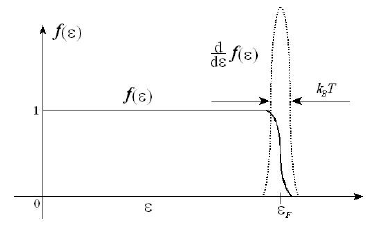
\includegraphics[scale=0.5]{fddash.png}
\end{figure}

\begin{example}[Calculate the Fermi energy and internal energy of a Fermi gas at temperature T up to order $T^2$.]
    We have
    \begin{align}
        g(\e)\;d\e &= \frac{4\pi V}{h^3}(2M)^{3/2} \e^{1/2}\,d\e
    \end{align}
    We need to evaluate $\e_F$ from
    \begin{align} 
        N &= \int_0^{\e_F} g(\e)f_{FD}(\e)\,d\e \approx \frac{2}{3}\mu^{3/2} + \frac{\pi^2}{12\beta^2\mu^{1/2}}
    \end{align}
    Then U follows from this.
\end{example}

What is the entropy of the Fermions?
At $T=0$, all Fermions have $S=0$, because there is only one way to arrange the Fermions.
Although we multiply by 2 for spin - this is only valid for systems which are not magnetic. 
Fermions carry a spin and hence are influenced by magnetic fields, even if the material is not \emph{magnetic}.
So applying a magnetic field to such a system gives us a \unl{paramagnet}.

Looking at the Ferm-Dirac distribution function:
If we apply $B$, then the up spins gain energy $+\mu_BB$ and the down spins gain energy $-\mu_BB$.
The distribution functions move left/right by energy $\mu_BB$.

Turning this into bands.
So the up spins flip to down spins (energy obtained from the $B$-field.
\emph{Double check this graph.}
\begin{figure}[H]
    \centering
    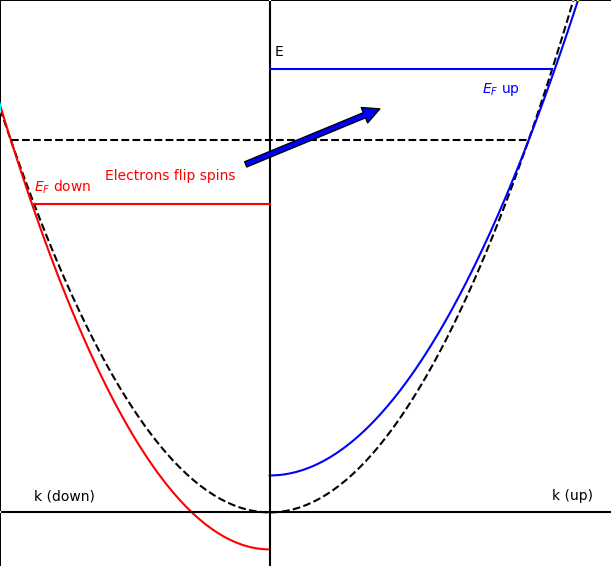
\includegraphics[scale=0.4]{elbnds.png}
\end{figure}

\chapter{}

\begin{example}
    $^3$He is a Fermion because it consists of 2 protons and 1 neutron and 2 electrons $\to$ 5 half-spin. 
    In the gas, it behaves classically so we use the Maxwell-Boltzmann distribution. However, in the liquid, the system is more interesting. 
    In the phase diagram of $^3$He, it remains liquid down to $T \approx 0$. 
    Note that at $T=0$, $S=0$, so liquid $^3$He has $S\approx0$ at $T\approx0$.
    \emph{Image in here}

    If we plot entropy vs temperatue, in the range where entropy of liquid is less than the solid. 
    \emph{Image in here}

    We've not considered zero point motion - $^3$He has low mass hence zero point motion may be significant. 
    Let's look at very low T phase diagram.
    \begin{figure}[H]
        \centering
        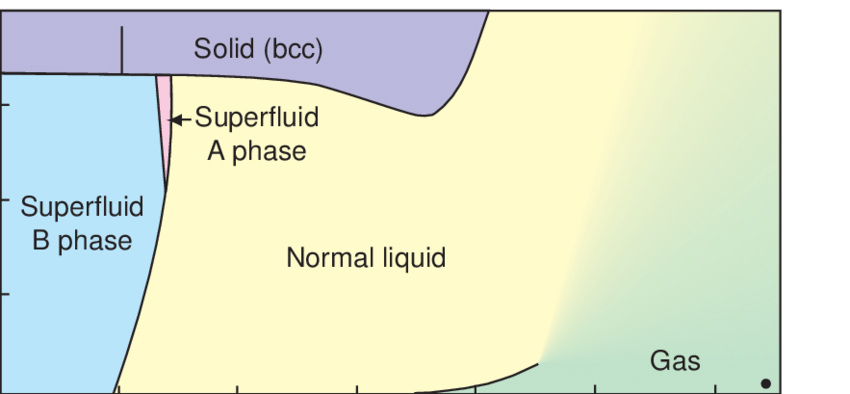
\includegraphics[scale=0.5]{he3.png}
    \end{figure}

    At low temperatures, $T\approx1\,$K, we get a liquid-liquid phase transition. 
    There is a very weak attraction between $^+$He atoms (spin-orbit interactions).
    The $^3$He atoms pair up - 2$^3$He:
    \begin{equation}
        |\uparrow\uparrow\rangle + |\downarrow\downarrow\rangle + \frac{1}{\sqrt{2}}|\uparrow\downarrow + \downarrow\uparrow\rangle
    \end{equation}
    This is a Boson.
    The Fermi particles $\to$ Bosons, hence they collapse down to the same ground state of the system, having a "macroscopic wavefunction".
\end{example}

A similar feature to the above occurs in some metals when they are cooled down. 
The electrons are Fermions and the usual conductivity physics happens. 
But if we pair them up into Bosons, then we get a similar Boson gas causing superconductivity. \\
We have positive ions in a sea of conducting electrons. 
The ions are slightly attracted to the path of an electron.
This positive path attracts a second electron causing coupling. 
This pair of eletrons is called a Cooper pair and is a Boson.
The electrons collapsie down into the Boson ground state giving superconductivity.

\section{Bose-Einstein Statistics}
The BE distribution is
\begin{equation}
    f_{BE}(\e) = \frac{1}{e^{\beta(\e-\mu)}-1}
\end{equation}
where $e^{\alpha} = e^{-\beta\mu}$ for particle number conservation and $\mu$ is the \unl{chemical potential} or Fermi level.
We have $g(\e)f_{BE}(\e)d\e$ is the number of particles in the energy range $\e \to \e+d\e$.
We must have
\begin{align}
    f_{BE}(\e) &> 1 \\
    e^{-\beta\mu}e^{\beta\e} &> 1 \\
    -\beta\mu + \beta\e &> 0 \\
    \mu &< \e \\
    \mu(T) &\leq 0
\end{align}
For Bosons at $T=0$, it is energetically favourable for all N of them to occupy the ground state.
Let $\e=0$ be the lowest energy state, so at $T=0$, we have
\begin{align}
    f_{BE}(0) &= N \\
    \frac{1}{e^{-\beta\mu}-1} &= N
\end{align}
For a low enough T, a macroscopic number of Bosons is in the ground state. 
Let this be $n_0(T)$.
Let $T_B$ be a low temperature where $n_0(T)$ is macroscopic, i.e. $n_0(T<T_B)$ is large.
\begin{align}
    n_0(T<T_B) \gg 1 \approx N
\end{align}
So for $T < T_B$, we have
\begin{align}
    \frac{1}{e^{-\beta\mu(T)}-1} &= n_0(T) \\
    e^{-\beta\mu(T)} &= 1 + \frac{1}{n_0(T)} \\
    -\beta\mu(T) &= \ln\left(1+\frac{1}{n_0(T)}\right) \approx \frac{1}{n_0(T)}, ~ [\ln(1+x) \approx x] \\
    \mu(T) &= -\frac{k_BT}{n_0(T)}
\end{align}
Since T is small, and $n_0(T)$ is big.

\subsection{Density of States}
Investigating the low T limit of density of states, we get:
\begin{align}
    N = \int_0^{\delta\e} g(\e)f_{BE}(\e)\,d\e &= C\int_0^{\delta\e} \sqrt{\e} \frac{1}{e^{-\beta\e} -1}\,d\e \\
                                               &= C\cancel{\delta\e}\frac{(\delta\e/2)^{1/2}}{\beta(\delta\e/2)} = 0
\end{align}
This is not correct - a problem!!

\chapter{}
\section{Bose-Einstein Condensation}
For bosons, $g(\e) \approx \sqrt{\e}$, so
\begin{equation}
    N = \int_0^{d\e} g(\e)f_{BE}(\e)\,d\e = 0
\end{equation}
We modify the DoS to allow all the particles to occupy the lowest energy state at $T=0$ - we do this by adding on a $\delta$-function, i.e. $g(\e) \to g(\e) + \delta(\e)$.
\begin{align}
    N = \int_0^{\delta\e} \delta(\e)f_{BE}(\e)\,d\e + \int_0^{\delta\e} g(\e)f_{BE}(\e)\,d\e &= \frac{1}{e^{-\beta\mu - 1}},~ \to N, T \to 0
\end{align}
Let's now calculate the number of bosons in the ground state at T, call this $n_0(T)$.
The total number of particles is the number in the ground state plus the rest:
\begin{align}
    N &= \underbrace{\frac{1}{e^{-\beta\mu}-1}}_{n_0(T)} + \underbrace{\ofnt g(\e)f_{BE}(\e)\,d\e}_{N^{th}(T)} \\ 
      &= n_0(T) + N^{th}(T)
\end{align}
So let's substitute in the usual $g(\e)$ to get:
\begin{align}
    N^{th}(T) &= \frac{2\pi V(2m)^{3/2}}{h^3} \ofnt \frac{\sqrt{\e}}{e^{-\beta\mu}e^{\beta\e}-1}d\e
\end{align}
Previously, we found that for some T, call it $T_B$, where $T<T_B$, $n_0(T)$ became macroscopic.
We know that at $T=0$, the Fermi level (chemical potential, $\mu$) is zero.
So continue with
\begin{align}
    N^{th}(T) &= \frac{2\pi V(2m)^{3/2}}{h^3} \ofnt \frac{\sqrt{\e}}{e^{\beta\e}-1}d\e
\end{align}
and if we substitute $x = \beta\e,~ dx = \beta\,d\e$, we get
\begin{align}
    N^{th}(T) &= \frac{2\pi V("M)^{3/2}}{(h^2\beta)^{3/2}} \ofnt \frac{\sqrt{x}}{e^x - 1}dx \\
\end{align}
\begin{itemize}
    \item \emph{Aside: This is a standard integral involving the Riemann-Zeta function:}
        \begin{align}
            \zeta(y) &= 1^{-y} + 2^{-y} + 3^{-y} + \cdots = \sum_{k=1}^\infty k^{-y} \\
            \ofnt \frac{\sqrt{x}}{e^x -1}dx &= \frac{\sqrt{\pi}}{2} ~\zeta\left(\frac{3}{2}\right) \approx 2.612\frac{\sqrt{\pi}}{2}
        \end{align}
\end{itemize}
So using this, 
\begin{align}
    N^{th}(T) &= 2\pi V\left(\frac{2M}{h^2\beta}\right)^{3/2}\frac{\sqrt{\pi}}{2}~\zeta\left(\frac{3}{2}\right) \\
              &= 2.612\frac{V}{h^3}(2\pi Mk_B)^{3/2}T^{3/2} \propto T^{3/2} \\
    N^{th}(T) &= \begin{cases} cT^{3/2} & T \leq T_B \\ \approx N & T > T_B \end{cases}
\end{align}
Let's investigate $T_B$.
For $T \leq T_B$, we get
\begin{align}
    \frac{n_0(T)}{N} &= \frac{N-N^{th}(T)}{N} = 1 - \frac{N^{th}(T)}{N} \\
                     &= 1 - \frac{c T^{3/2}}{c T_B^{3/2}} \\
    n_0(T) &= N\left(1 - \left(\frac{T}{T_B}\right)^{3/2}\right)
\end{align}
As the temperature drops below $T_B$, there is a sudden and rapid increase in the population of the ground state, $\e = 0$, and at $T=0$, $n_0(T) = N$.
This is known as \emph{Bose-Einstein condensation.}

\subsection{Internal Energy}
For $T \leq T_B$, the internal energy is
\begin{align}
    U(T) &= \cancel{\ofnt \e\delta(\e)f_{BE}(\e)\,d\e} + \frac{2\pi V}{h^3}(2M)^{3/2} \ofnt \e\sqrt{\e}f_{BE}(\e)\,d\e
\end{align}
So the "condensate" does not contribute to the internal energy of the system.
Hence, 
\begin{align}
    U(T) &= \frac{2\pi V}{h^3}(2M)^{3/2}\ofnt \e^{3/2}f_{BE}(\e)\,d\e
\end{align}
\begin{itemize}
    \item Note that:
        \begin{equation}
            \ofnt \frac{x^{3/2}}{e^x -1}dx = \frac{3}{4}\sqrt{\pi}~\zeta\left(\frac{5}{2}\right) \approx 1.783
        \end{equation}
\end{itemize}
So this gives
\begin{align}
    U(T) &= \frac{2.012V}{h^3}(2\pi M)^{3/2}(k_BT)^{5/2}
\end{align}
So we have $U(T) \propto T^{5/2}$ and hence $C_V \propto T^{3/2}$.
Recall from thermodynamics, $P \propto \frac{U}{V}$ and so $P \propto T^{5/2}$.

\begin{example}
    $^4$He is $2p + 2n + 2e$ hence is a boson.
    It remains fluid at $T=0$ and there is a phase transition at $T\approx 2$K.
    \begin{figure}[H]
        \centering
        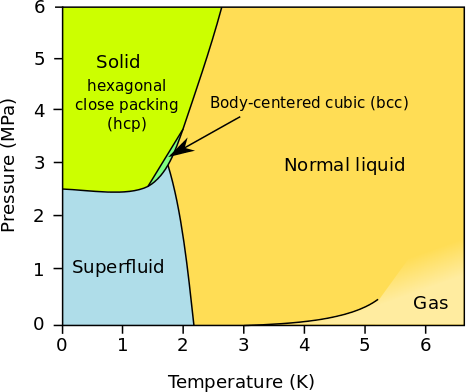
\includegraphics[scale=0.4]{he4.png}
        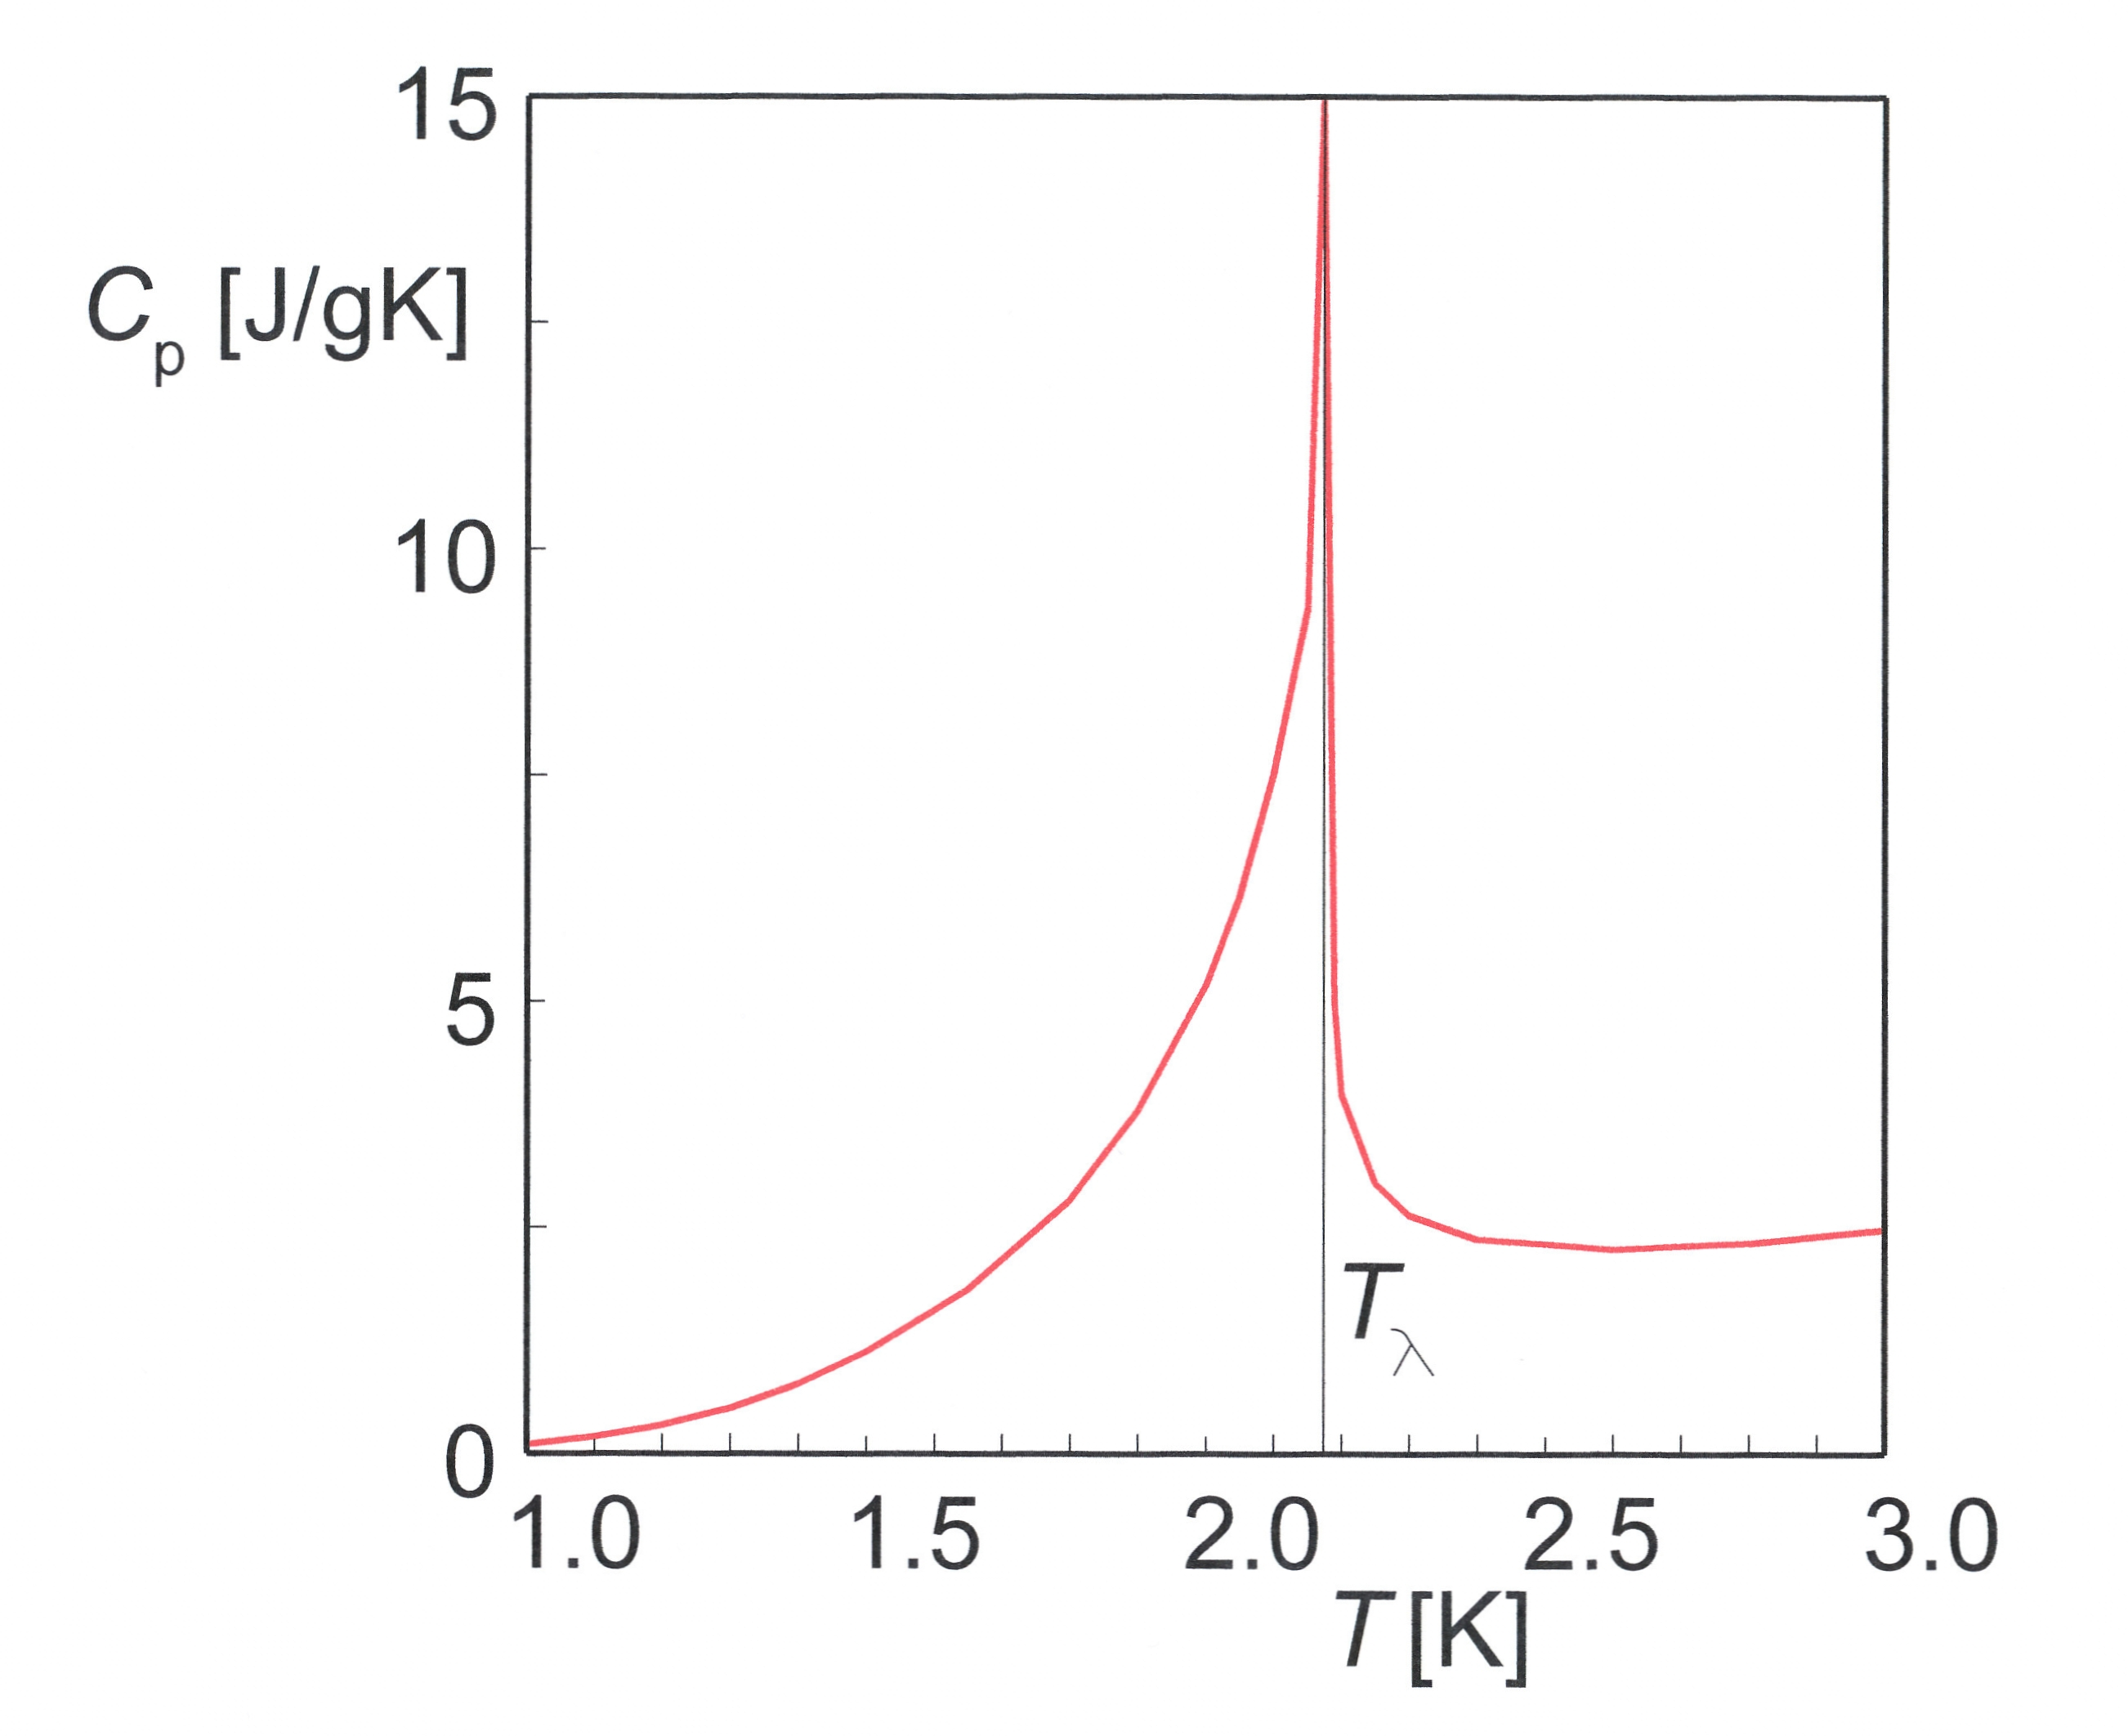
\includegraphics[scale=0.4]{h4cv.jpg}
    \end{figure}
    The divergence in $C_V$ implies a phase transition.
\end{example}

\chapter{}
\section{Photons and Phonons (Bosons)}
Photons do not interact with each other. 
This is why we can see emission from billions of years ago. 
Photons and phonons are particles obeying BE statistics, and it costs zero energy to add or remove one. 
There, the chemical potential is zero. 
The mass of these Bosons is zero:
\begin{itemize}
    \item BLackbody radiation
    \item Lattice vibrations
        \begin{itemize}
            \item Both of these exist at a temperature $T$ in a volume $V$
        \end{itemize}
\end{itemize}
As the chemical potential is zero, we have no Lagrange multiplier constraining particle number. 
Hence, the distribution function is
\begin{equation}
    f_{BE}(\e) = \frac{1}{e^{\beta\e} - 1}
\end{equation}
Also, we have $\e = \hbar\om = h\nu$. 

The average energy per photon/phonon is the average number of photons per state ($f_{BE}(x)$) times the average energy of the photon/phonon,
\begin{equation}
    \frac{U}{N} = \frac{\hbar\om}{e^{\beta\hbar\om}-1}.
\end{equation}
However, we know that oscillators have energies, $\e_n = n\hbar\om,~ n \in \N$.

Consider an oscillator which has groun state, $\e_0 = 0$, and first excited state $\e_i = \hbar\om$.
If there are n Bosons in the excited state then energy is $n\hbar\om$.
This is the same as having one Boson in state $n$.
Collections of Bosons act as groups of oscillators that have the same energy as a single particle.

\section{Spectral Density}
For such systems, it is often more convenient to use density of states $g(\om)$ rather than $g(\e)$, i.e. the number of states in $\om \to \om+d\om$ is $g(\om)d\om$.
Energy:
\begin{equation}
    \int g(\om)\,d\om\, f(\om)\hbar\om = U
\end{equation}
In k-space, this is usually a general starting point as it is independent of particle type, i.e.
\begin{equation}
    g(k)\delta k = \frac{V}{(2\pi)^3}4\pi^2k^2\delta k \times 2
\end{equation}
The multiplication by 2 is analagous to degrees of freedom - photons have two independent transverse polarisations. 
We have $c = \frac{\om}{k}$, $c = \nu\lambda$, we get $dk = \frac{d\om}{c}$.

This gives Planck's Radiation Formula:
\begin{equation}
    g(\om)f(\om)d\om = \frac{\hbar V}{\pi^2c^3} \om^3 d\om \frac{1}{e^{\beta\hbar\om}-1}
\end{equation}
or
\begin{equation}
    g(\nu)d\nu = \frac{8\pi hV}{c^3}\nu^3d\nu \frac{1}{e^{\beta h\nu}-1}.
\end{equation}
From this, other properties follow, such as Wien's Displacement Law, Stefan-Boltzmann, etc.
Total energy:
\begin{align}
    \frac{U}{N} &= \frac{8\pi hV}{c^3} \ofnt \frac{v^3}{e^{\beta h\nu}-1}d\nu,~ x = \beta h\nu \\
                &= \frac{8\pi V}{c^3\beta^4h^3} \underbrace{\ofnt \frac{x^3}{e^x - 1}dx}_{\pi^4/15} = \underbrace{\frac{8\pi^5Vk_B^4}{15c^3h^3}}_{\text{Stefan constant, }\sigma}T^4
\end{align}

\section{Radiation Pressure}
From $dU = TdS - pdV$,
\begin{equation}
    p = -\left(\frac{\p U}{\p V}\right)_S
\end{equation}
As S depends on occupation number, 
\begin{equation}
    \{n_i\} \implies p = -\left(\frac{\p U}{\p V}\right)_S = -\sum_i \frac{\p\e_i}{\p V}
\end{equation}
But $\e_i \propto V^{-2/3}$. 
Remember that
\begin{align}
    \e_n &= \frac{n^2\pi^2\hbar^2}{2m} \\
    \implies p &= \frac{2}{3}\sum_i n_i\frac{\e_i}{V} = \frac{2}{3}\frac{U}{V}
\end{align}
How many photons per unit volume in a cavity at temperature, $T$?
\begin{align}
    N &= \ofnt g(\nu)f(\nu)d\nu \\
    \implies \frac{N}{V} &= \frac{8\pi}{c^3h^3\beta} \ofnt \frac{x^2}{e^x - 1}dx \\
                         &= 60.42 \frac{k_B^3}{c^3h^3}T^3
\end{align}
Much of the above applies to phonons. 
Differences are phonons have 3 polarisations (2 transverse, 1 longitudinal), and the dispersion curves are more complicated.
\begin{figure}[H]
    \centering
    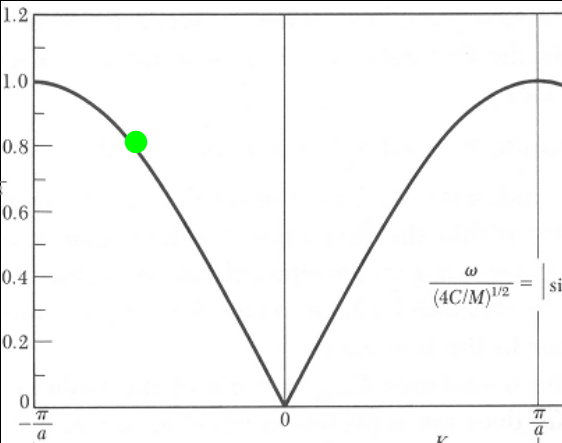
\includegraphics[scale=0.5]{brill.png}
\end{figure}

\chapter{}
\section{Entropy}
Let $S_m$ be the entropy of an m particle system, and probabilities of particles being in the allowed states be $\{p_i\}$.
Properties:
\begin{enumerate}
    \item $S_m(\{p_i\}) \geq 0$
    \item Permutation invariance -
        \begin{equation}
            S_m(p_1,p_2,\dots,p_m) = S_m(p_2,p_1,\dots,p_m)
        \end{equation}
    \item Expansible -
        \begin{equation}
            S_m(p_1,p_2,\dots,p_m,0) = S_m(p_1,p_2,\dots,p_m)
        \end{equation}
    \item Normalisable - 
        \begin{equation}
            S_2\left(\frac{1}{2},\frac{1}{2}\right) = \text{constant}
        \end{equation}
    \item Additivity (if $x$ and $y$ are independent) - 
        \begin{equation}
            S(x,y) = S(x) + S(y)
        \end{equation}
    \item Continuity -
        \begin{equation}
            S_2(p,1-p) \to 0, p \to 0
        \end{equation}
\end{enumerate}
It has been proven (elsewhere) that all of these can be satisfied only with 
\begin{equation}
    S_m = -\sum_i p_i\ln(p_i).
\end{equation}
But what if there is some other property that satisfies these conditions?

\subsection{Let's Play A Game}
\begin{example}
    We have scrabble tiles with only 4 letters A,B,C, and D in equal quantities. 
    How many yes/no questions do I have to ask to determine what a randomly picked tile is?
    \begin{itemize}
        \item AB (50\%) or CD (50\%)?
            \begin{itemize}
                \item A (25\%) or B (25\%)?
                \item C (25\%) or D (25\%)?
            \end{itemize}
    \end{itemize}
    This can be modelled in bits, where one would only need 2 bits to get an answer - (00, 01, 10, 11).

    What if the bag had 50\% A, 25\% B, and 12.5\% for both C and D?
    \begin{itemize}
        \item A (50\%) or BCD (50\%)?
            \begin{itemize}
                \item B (25\%) or CD (25\%)?
                    \begin{itemize}
                        \item C (25\%) or D (25\%)?
                    \end{itemize}
            \end{itemize}
    \end{itemize}
    To find out a tile's identity, we ask 1 question half the time, 2 questions a quarter of the time, and 3 questions an eighth of the time - 1.75 questions on average. 

    Let's define information content as the number of questions that need to asked. 
    \begin{equation}
        \text{Information} = \sum_i p_i \times \text{number of questions of level }i
    \end{equation}
    \emph{Level i is the level of the tree we're on.}
    \begin{align}
        \text{Number of questions given by level i} &= \log_2(\underbrace{\text{questions on tree}}_{1/p}) \\
        \text{Information} &= \sum_i p_i\log_2\frac{1}{p_i} = -\sum_i p_i\log_2p_i
    \end{align}
    \begin{itemize}
        \item Problem 2 has an entropy of 1.75
        \item Problem 1 has an entropy of 2
    \end{itemize}
    So Problem 1 has a higher entropy. 
    The more disordered a system is, the more information it contains. 

    Another game: 12 balls looking all the same, but 1 is heavier or lighter (we don't know). 
    Using balance scales, what's the minimum number of measurements to identify the odd ball?

    The slowest way to do this is to compare each ball one by one, i.e. 12 tries. 
    The better way would be to maximise entropy. 
    Get the maximum amount of information at each step.
\end{example}

\section{Entropy of the Universe}
If you played a movie, and it looked the same forward and backward, then you can't tell what the arrow of time is. 
Most physical laws are time reversible, entropy gives us the arrow of time. 
\end{document}
